\begin{practice}
    \subsection{Luyện tập}

    \begin{questions}[series=SBT]
        \item Tính đến hết SEA Games 32 đã có năm quốc gia từng lên ngôi vô địch bóng đá nam SEA Games, cụ thể như sau:

        \begin{center}
        \begin{tblr}{
            width=\linewidth,
            colspec={Q[l,3cm] X[l]},
            row{1}={font=\bfseries, halign=c},
            cells={valign=m}
        }
            Đội tuyển & Năm vô địch \\
            Thái Lan & 1975, 1981, 1983, 1985, 1993, 1995, 1997, 1999, 2001, 2003, 2005, 2007, 2013, 2015, 2017 \\
            Malaysia & 1961, 1977, 1979, 1989, 2009, 2011 \\
            Myanmar & 1965, 1967, 1969, 1971, 1973 \\
            Việt Nam & 1959; 2019, 2021 \\
            Indonesia & 1987, 1991, 2023 \\
        \end{tblr}
        \end{center}

        \begin{flushright}
            \textit{(Theo sportingnews.com)}
        \end{flushright}

        \begin{questions}
            \item Lập bảng tần số biểu diễn số lần vô địch môn bóng đá nam SEA Games của các quốc gia trên.

            \answerline
            \answerline

            \item Từ bảng tần số thu được ở câu a, hãy cho biết quốc gia nào vô địch môn Bóng đá nam SEA Games nhiều nhất, với mấy lần vô địch.

            \answerline
        \end{questions}

        \item Giáo viên dạy Toán ghi lại số bài tập mỗi học sinh trong lớp đã làm sau bài học tuần trước cho kết quả như sau:

        \[
        \begin{aligned}
            &4,\ 2,\ 0,\ 5,\ 4,\ 3,\ 2,\ 1,\ 3,\ 3,\ 6,\ 1,\ 3,\ 2,\ 4,\ 3,\ 5,\ 3,\\
            &3,\ 1,\ 4,\ 6,\ 1,\ 2,\ 3,\ 5,\ 3,\ 2,\ 4,\ 3,\ 1,\ 4,\ 4,\ 5,\ 6,\ 2.
        \end{aligned}
        \]

        \begin{questions}
            \item Lập bảng tần số cho dãy số liệu trên.

            \answerline
            \answerline

            \item Có bao nhiêu bạn trong lớp làm ít nhất ba bài tập?

            \answerline
        \end{questions}

        \item Bảng sau cho biết kết quả bình chọn môn thể thao được yêu thích nhất của các bạn học sinh lớp 9A (mỗi gạch biểu diễn cho một bạn bình chọn):

        \begin{center}
        \begin{tblr}{
            colspec={Q[l,3cm] Q[l,7cm]},
            cells={valign=m}
        }
            Bóng đá & {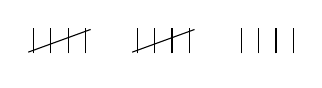
\begin{tikzpicture}[x=0.22cm,y=0.32cm,baseline=-0.5ex]
                \foreach \s in {0,1} {
                    \foreach \x in {0,1,2,3} \draw (\s*6+\x,0)--(\s*6+\x,1);
                    \draw (\s*6-0.3,0.05)--(\s*6+3.3,0.95);
                }
                \foreach \x in {12,13,14,15} \draw (\x,0)--(\x,1);
            \end{tikzpicture}} \\
            Cầu lông & {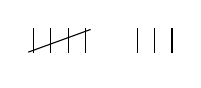
\begin{tikzpicture}[x=0.22cm,y=0.32cm,baseline=-0.5ex]
                \foreach \x in {0,1,2,3} \draw (\x,0)--(\x,1);
                \draw (-0.3,0.05)--(3.3,0.95);
                \foreach \x in {6,7,8} \draw (\x,0)--(\x,1);
            \end{tikzpicture}} \\
            Bóng bàn & {\begin{tikzpicture}[x=0.22cm,y=0.32cm,baseline=-0.5ex]
                \foreach \x in {0,1,2,3} \draw (\x,0)--(\x,1);
            \end{tikzpicture}} \\
            Môn khác & {\begin{tikzpicture}[x=0.22cm,y=0.32cm,baseline=-0.5ex]
                \foreach \x in {0,1,2,3} \draw (\x,0)--(\x,1);
                \draw (-0.3,0.05)--(3.3,0.95);
                \foreach \x in {6,7} \draw (\x,0)--(\x,1);
            \end{tikzpicture}} \\
        \end{tblr}
        \end{center}

        \begin{questions}
            \item Lập bảng tần số cho kết quả bình chọn trên.

            \answerline
            \answerline

            \item Dựa vào bảng tần số thu được ở câu a, cho biết môn thể thao nào được các bạn yêu thích nhất.

            \answerline
        \end{questions}

        \item Biểu đồ sau cho biết kết quả khảo sát trình độ tiếng Anh của sinh viên cuối năm thứ nhất ở một trường đại học:

        \begin{center}
        \begin{tikzpicture}[x=1.35cm,y=0.024cm]
            \foreach \y in {0,50,100,150,200,250,300,350,400} {
                \draw[base200] (0,\y)--(6,\y);
                \node[left] at (0,\y) {\y};
            }
            \draw[->] (0,0)--(6.2,0);
            \draw[->] (0,0)--(0,420);
            \foreach \x/\lab in {0.7/A1,1.8/A2,2.9/B1,4.0/B2,5.1/C1} {
                \node[below] at (\x,0) {\lab};
            }
            \foreach \x/\h in {0.7/102,1.8/115,2.9/345,4.0/35,5.1/3} {
                \fill[base700] (\x-0.23,0) rectangle (\x+0.23,\h);
                \node[above] at (\x,\h) {\h};
            }
            \node[font=\bfseries,align=center] at (3,470) {Kết quả khảo sát trình độ tiếng Anh của sinh viên\\cuối năm thứ nhất};
            \node[below] at (3,-55) {Trình độ tiếng Anh};
            \node[rotate=90] at (-0.85,210) {Số sinh viên};
        \end{tikzpicture}
        \end{center}

        \begin{questions}
            \item Đọc và giải thích số liệu được biểu diễn trên hai cột bất kì của biểu đồ.

            \answerline

            \item Lập bảng tần số cho dữ liệu được biểu diễn trên biểu đồ.

            \answerline
            \answerline

            \item Để tốt nghiệp đại học, sinh viên cần có trình độ tiếng Anh ở mức B1 trở lên. Ước lượng tỉ lệ sinh viên cuối năm thứ nhất đã đạt chuẩn trình độ tiếng Anh.

            \answerline
            \answerline
        \end{questions}

        \item Số $\pi$ với 50 chữ số sau dấu phẩy thập phân như sau:

        \[
            3{,}141\ 592\ 653\ 589\ 793\ 238\ 462\ 643\ 383\ 279\ 502\ 884\ 197\ 169\ 399\ 375\ 10.
        \]

        \begin{questions}
            \item Lập bảng tần số cho các chữ số từ 0 đến 9 xuất hiện sau dấu phẩy thập phân.

            \answerline
            \answerline

            \item Chữ số nào xuất hiện nhiều nhất, ít nhất?

            \answerline
        \end{questions}

        \item Cho biểu đồ tần số dạng đoạn thẳng sau:

        \begin{center}
        \begin{tikzpicture}[x=1.25cm,y=0.45cm]
            \foreach \y in {0,2,4,6,8,10,12,14} {
                \draw[base200] (0,\y)--(7,\y);
                \node[left] at (0,\y) {\y};
            }
            \draw[->] (0,0)--(7.2,0);
            \draw[->] (0,0)--(0,15);
            \foreach \x/\lab in {1/5,2/6,3/7,4/8,5/9,6/10} {
                \node[below] at (\x,0) {\lab};
            }
            \draw[base700,thick] (1,2)--(2,6)--(3,10)--(4,13)--(5,7)--(6,1);
            \foreach \x/\h in {1/2,2/6,3/10,4/13,5/7,6/1} {
                \draw[fill=white] (\x,\h) circle (2.5pt);
                \node[above right] at (\x,\h) {\h};
            }
            \node[font=\bfseries] at (3.5,16.5) {Kết quả kiểm tra môn Toán};
            \node[below] at (3.5,-1.5) {Điểm};
            \node[rotate=90] at (-0.85,7.5) {Số học sinh};
        \end{tikzpicture}
        \end{center}

        \begin{questions}
            \item Lập bảng tần số cho dữ liệu được biểu diễn trên biểu đồ.

            \answerline
            \answerline

            \item Điểm nào có nhiều học sinh đạt nhất?

            \answerline
        \end{questions}

        \item Một túi chứa một số viên bi có cùng kích thước, mỗi viên bi có một trong các màu đen, trắng, đỏ, vàng. Thực hiện lấy bi 20 lần, mỗi lần lấy một viên xem viên bi có màu gì sau đó trả bi lại túi, trộn đều. Kết quả trong 20 lần lấy bi có 8 lần lấy được bi đen, 4 lần lấy được bi đỏ, 6 lần lấy được bi trắng, 2 lần lấy được bi vàng.

        \begin{questions}
            \item Lập bảng tần số cho kết quả thu được.

            \answerline
            \answerline

            \item Vẽ biểu đồ tần số dạng cột biểu diễn bảng tần số thu được ở câu a.

            \answerline
            \answerline
            \answerline
        \end{questions}

        \item Thống kê số ngày nằm viện của 20 bệnh nhân được kết quả như sau:

        \[
            5,\ 7,\ 4,\ 6,\ 8,\ 10,\ 6,\ 7,\ 8,\ 8,\ 6,\ 5,\ 8,\ 5,\ 4,\ 6,\ 5,\ 7,\ 4,\ 6.
        \]

        \begin{questions}
            \item Lập bảng tần số cho dãy số liệu trên.

            \answerline
            \answerline

            \item Vẽ biểu đồ tần số dạng đoạn thẳng biểu diễn bảng tần số thu được ở câu a.

            \answerline
            \answerline
            \answerline
        \end{questions}
    \end{questions}
\end{practice}
